\section{Lattice Vibrations \& Phonons}
\subsection{Phonons in One Dimension}
We consider a simple monoatomic chain:
\begin{figure}[htbp]
    \centering
    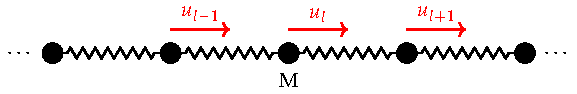
\includegraphics[]{Images/fig-monochaincartoon.pdf}

    \caption{A monoatomic chain. The atoms are of mass $M$ and are labelled with index $l$, with $u_l$ denoting the $l$th-atoms' displacement from equilibrium.}
    \label{fig-monochaincartoon}
\end{figure}
We label the atoms by index $l$ and the displacements from equilibrium for the $l$th atom by $u_l$. We assume we have a crystal lattice with individual atoms oscillating around equilibrium positions. The general Hamiltonian we can write for this system is:
\begin{equation}
    \begin{split}
        &H = \sum_l \frac{p_l^2}{2M} + V(u_1, u_2, \ldots)
        \\ &p_l = -i\hbar\dpd{}{u_l}
        \\ &[u_l, p_{l'}] = i\hbar\delta{ll'} 
    \end{split}
\end{equation}
Where we take the momentum to be canonically conjugate to the displacement and hence it satisfies the canonical commutation relation. We assume that the potential has a minimum for $u_l = 0$ for all $l$. We expand $V$ in a Taylor series about these minima:
\begin{equation}\label{eq-Vtaylor}
    V(u_1, u_2, \ldots) = V(0, 0, \ldots ) + \sum_l u_l \left[\dpd{V}{u_l}\right]_{u_1=u_2=\ldots = 0} + \frac{1}{2!}\sum_{l, l'}u_lu_{l'}\left[\frac{\partial^2 V}{\partial \mu_l \partial \mu_{l'}}\right]_{u_1=u_2=\ldots=0} + \frac{1}{3!} \ldots
\end{equation}
The first term can be eliminated by suitable choice of energy zero (a constant in the Hamiltonian changes none of the physics). The second term vanishes by virtue of $u_1 = u_2 = \ldots = 0$ being a minimum of $V$. We are left with just the second-order term, and so:
\begin{equation}
    H \approx \sum_l \frac{p_l^2}{2M} + \frac{1}{2}\sum_{l, l'}u_l V_{ll'}u_{l'}
\end{equation}
where $V_{ll'} = \left[\frac{\partial^2 V}{\partial \mu_l \partial \mu_{l'}}\right]_{u_1=u_2=\ldots=0}$ is the dynamical matrix. We neglect all higher order terms in Eq. \eqref{eq-Vtaylor} which amounts to a harmonic approximation.

Next day: we will show how to diagonalize this Hamiltonian and write it in second quantization. This gives us the basic theory of phonons various dispersion relations and physical observables that follow from these.